% Options for packages loaded elsewhere
\PassOptionsToPackage{unicode}{hyperref}
\PassOptionsToPackage{hyphens}{url}
\PassOptionsToPackage{dvipsnames,svgnames,x11names}{xcolor}
%
\documentclass[
  letterpaper,
  DIV=11,
  numbers=noendperiod,
  oneside]{scrartcl}

\usepackage{amsmath,amssymb}
\usepackage{iftex}
\ifPDFTeX
  \usepackage[T1]{fontenc}
  \usepackage[utf8]{inputenc}
  \usepackage{textcomp} % provide euro and other symbols
\else % if luatex or xetex
  \usepackage{unicode-math}
  \defaultfontfeatures{Scale=MatchLowercase}
  \defaultfontfeatures[\rmfamily]{Ligatures=TeX,Scale=1}
\fi
\usepackage{lmodern}
\ifPDFTeX\else  
    % xetex/luatex font selection
\fi
% Use upquote if available, for straight quotes in verbatim environments
\IfFileExists{upquote.sty}{\usepackage{upquote}}{}
\IfFileExists{microtype.sty}{% use microtype if available
  \usepackage[]{microtype}
  \UseMicrotypeSet[protrusion]{basicmath} % disable protrusion for tt fonts
}{}
\makeatletter
\@ifundefined{KOMAClassName}{% if non-KOMA class
  \IfFileExists{parskip.sty}{%
    \usepackage{parskip}
  }{% else
    \setlength{\parindent}{0pt}
    \setlength{\parskip}{6pt plus 2pt minus 1pt}}
}{% if KOMA class
  \KOMAoptions{parskip=half}}
\makeatother
\usepackage{xcolor}
\usepackage[left=1in,marginparwidth=2.0666666666667in,textwidth=4.1333333333333in,marginparsep=0.3in]{geometry}
\setlength{\emergencystretch}{3em} % prevent overfull lines
\setcounter{secnumdepth}{5}
% Make \paragraph and \subparagraph free-standing
\makeatletter
\ifx\paragraph\undefined\else
  \let\oldparagraph\paragraph
  \renewcommand{\paragraph}{
    \@ifstar
      \xxxParagraphStar
      \xxxParagraphNoStar
  }
  \newcommand{\xxxParagraphStar}[1]{\oldparagraph*{#1}\mbox{}}
  \newcommand{\xxxParagraphNoStar}[1]{\oldparagraph{#1}\mbox{}}
\fi
\ifx\subparagraph\undefined\else
  \let\oldsubparagraph\subparagraph
  \renewcommand{\subparagraph}{
    \@ifstar
      \xxxSubParagraphStar
      \xxxSubParagraphNoStar
  }
  \newcommand{\xxxSubParagraphStar}[1]{\oldsubparagraph*{#1}\mbox{}}
  \newcommand{\xxxSubParagraphNoStar}[1]{\oldsubparagraph{#1}\mbox{}}
\fi
\makeatother


\providecommand{\tightlist}{%
  \setlength{\itemsep}{0pt}\setlength{\parskip}{0pt}}\usepackage{longtable,booktabs,array}
\usepackage{calc} % for calculating minipage widths
% Correct order of tables after \paragraph or \subparagraph
\usepackage{etoolbox}
\makeatletter
\patchcmd\longtable{\par}{\if@noskipsec\mbox{}\fi\par}{}{}
\makeatother
% Allow footnotes in longtable head/foot
\IfFileExists{footnotehyper.sty}{\usepackage{footnotehyper}}{\usepackage{footnote}}
\makesavenoteenv{longtable}
\usepackage{graphicx}
\makeatletter
\def\maxwidth{\ifdim\Gin@nat@width>\linewidth\linewidth\else\Gin@nat@width\fi}
\def\maxheight{\ifdim\Gin@nat@height>\textheight\textheight\else\Gin@nat@height\fi}
\makeatother
% Scale images if necessary, so that they will not overflow the page
% margins by default, and it is still possible to overwrite the defaults
% using explicit options in \includegraphics[width, height, ...]{}
\setkeys{Gin}{width=\maxwidth,height=\maxheight,keepaspectratio}
% Set default figure placement to htbp
\makeatletter
\def\fps@figure{htbp}
\makeatother

\KOMAoption{captions}{tableheading}
\makeatletter
\@ifpackageloaded{caption}{}{\usepackage{caption}}
\AtBeginDocument{%
\ifdefined\contentsname
  \renewcommand*\contentsname{Table of contents}
\else
  \newcommand\contentsname{Table of contents}
\fi
\ifdefined\listfigurename
  \renewcommand*\listfigurename{List of Figures}
\else
  \newcommand\listfigurename{List of Figures}
\fi
\ifdefined\listtablename
  \renewcommand*\listtablename{List of Tables}
\else
  \newcommand\listtablename{List of Tables}
\fi
\ifdefined\figurename
  \renewcommand*\figurename{Figure}
\else
  \newcommand\figurename{Figure}
\fi
\ifdefined\tablename
  \renewcommand*\tablename{Table}
\else
  \newcommand\tablename{Table}
\fi
}
\@ifpackageloaded{float}{}{\usepackage{float}}
\floatstyle{ruled}
\@ifundefined{c@chapter}{\newfloat{codelisting}{h}{lop}}{\newfloat{codelisting}{h}{lop}[chapter]}
\floatname{codelisting}{Listing}
\newcommand*\listoflistings{\listof{codelisting}{List of Listings}}
\makeatother
\makeatletter
\makeatother
\makeatletter
\@ifpackageloaded{caption}{}{\usepackage{caption}}
\@ifpackageloaded{subcaption}{}{\usepackage{subcaption}}
\makeatother
\makeatletter
\@ifpackageloaded{sidenotes}{}{\usepackage{sidenotes}}
\@ifpackageloaded{marginnote}{}{\usepackage{marginnote}}
\makeatother

\ifLuaTeX
  \usepackage{selnolig}  % disable illegal ligatures
\fi
\usepackage{bookmark}

\IfFileExists{xurl.sty}{\usepackage{xurl}}{} % add URL line breaks if available
\urlstyle{same} % disable monospaced font for URLs
\hypersetup{
  pdftitle={Assignment\_TV show report},
  pdfauthor={Lian Yutong},
  colorlinks=true,
  linkcolor={blue},
  filecolor={Maroon},
  citecolor={Blue},
  urlcolor={Blue},
  pdfcreator={LaTeX via pandoc}}


\title{Assignment\_TV show report}
\author{Lian Yutong}
\date{}

\begin{document}
\maketitle

\renewcommand*\contentsname{Table of contents}
{
\hypersetup{linkcolor=}
\setcounter{tocdepth}{2}
\tableofcontents
}
\listoffigures

\section{Introduction}\label{introduction}

\emph{Suits} is an American television drama series created by Aaron
Korsh, which premiered on June 23, 2011, on the USA Network. It revolves
around Mike Ross (Patrick J. Adams), who begins working as a law
associate for Harvey Specter (Gabriel Macht), despite never attending
law school. The show focuses on Harvey and Mike managing to close cases,
while maintaining Mike's secret.

The series was renewed for an eighth season on January 30, 2018. In
January 2019, the series was renewed for a ninth and final season which
premiered on July 17, 2019. During the course of the series, 134
episodes of \emph{Suits} aired over nine seasons, between June 23, 2011,
and September 25, 2019.

\begin{center}

\includegraphics{images/suits-01.jpg}
\end{center}

\section{Viewership}\label{viewership}

\subsection{Viewership Over Time}\label{viewership-over-time}

\begin{itemize}
\item
  \textbf{Season 1 (2011)}:\\
  The premiere attracted approximately \textbf{4.64} million viewers.
\item
  \textbf{Season 2 (2012)}:\\
  The premiere had about \textbf{3.47} million viewers.
\item
  \textbf{Season 3 (2013)}:\\
  The premiere had about\textbf{2.93} million viewers.
\item
  \textbf{Season 4 (2014-2015):}\\
  The premiere had about \textbf{2.50} million viewers.
\item
  \textbf{Season 5 (2015--2016)}:\\
  The premiere had about \textbf{2.13} million viewers.
\item
  \textbf{Season 6 (2016--2017)}:\\
  The premiere had about \textbf{1.85} million viewers.
\item
  \textbf{Season 7 (2017-2018):}\\
  The premiere had about \textbf{1.40} million viewers.
\item
  \textbf{Season 8 (2018-2019):}\\
  The premiere had about \textbf{1.27} million viewers.
\item
  \textbf{Season 9 (2019-2020)}:\\
  The premiere had about \textbf{1.04} million viewers.
\end{itemize}

Source: \url{https://en.wikipedia.org/wiki/Suits_(American_TV_series)}

Overall, \emph{Suits} started strong in its early seasons but saw a
gradual decline in ratings over time.\\
However, it achieved incredible success on streaming platforms later,
becoming one of the most-watched series in 2023, with nearly 57.7
billion minutes streamed. (Source:
\href{https://www.facebook.com/TheBoardroom/posts/originally-airing-from-2011-to-2019-suits-built-a-loyal-fanbase-during-its-nine-/1133161235490015/?utm_source=chatgpt.com}{facebook.com})

\begin{verbatim}
Warning: package 'ggplot2' was built under R version 4.4.3
\end{verbatim}

\begin{figure*}

\begin{minipage}{0.50\linewidth}

\begin{figure}[H]

{\centering 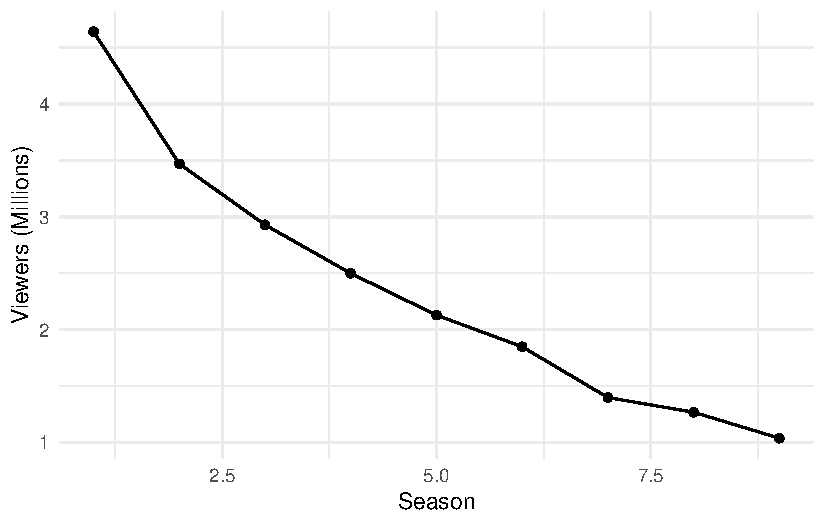
\includegraphics{Assignment_TV-Show_files/figure-pdf/unnamed-chunk-1-1.pdf}

}

\subcaption{Suits Viewership Over seasons}

\end{figure}%

\end{minipage}%
%
\begin{minipage}{0.50\linewidth}

\begin{figure}[H]

{\centering 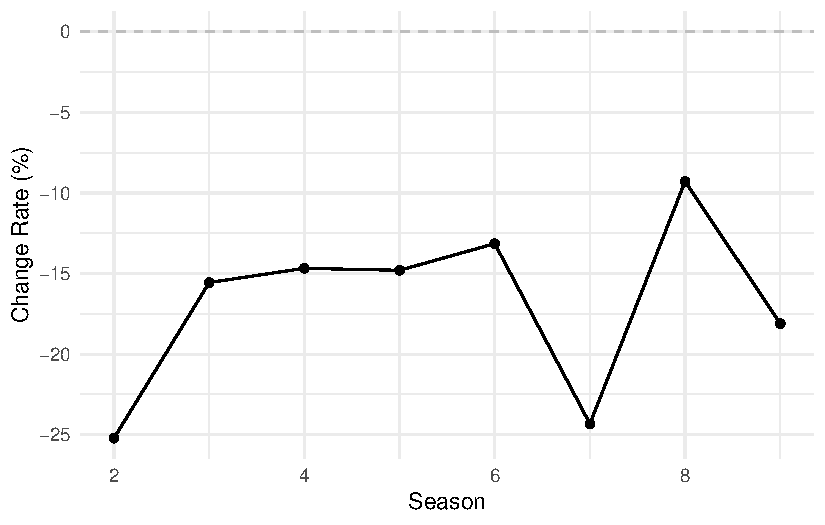
\includegraphics{Assignment_TV-Show_files/figure-pdf/unnamed-chunk-1-2.pdf}

}

\subcaption{Suits change rate of Viewership Over seasons}

\end{figure}%

\end{minipage}%

\end{figure*}%

Between Season 1 and Season 3, the viewership dropped from 4.64 million
to 2.93 million, a decrease of approximately 1.71 million viewers.From
Season 3 to Season 5, the viewership declined from 2.93 million to 2.13
million, a loss of around 0.8 million viewers.The sharpest decline
occurred between Season 6 and Season 7, with a drop from 1.85 million to
1.4 million, about 0.45 million viewers.Overall, from Season 1 to Season
9, the viewership decreased by about 3.6 million viewers.




\end{document}
